\chapter{Application to HCP pre-processing pipelines}

\section{Data}
\paragraph{HCP Data Acquisition}
The data was acquired from Human Connectome Project\footnote{\url{https://db.humanconnectome.org}}. We used the subjects 101006, 101017, 101410, 104820 and 105216. All these subjects were scanned using the HCP3T type of scanner. Figures \ref{fig:subject_details} and \ref{fig:subject_scan_details} gives more insight about the HCP subjects that were used for our study. 

\begin{center}
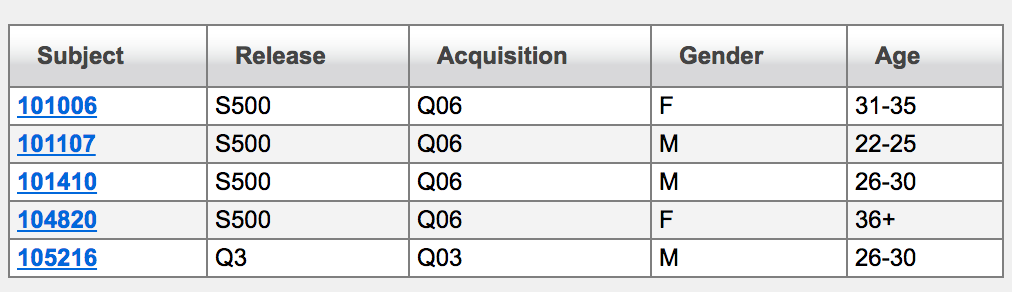
\includegraphics[width=\linewidth]{subjects_details.png}
\captionof{figure}{Subject Details}
\label{fig:subject_details}
\caption*{Extracted from \cite{DBConnectomeSite}}
\end{center}

\begin{center}
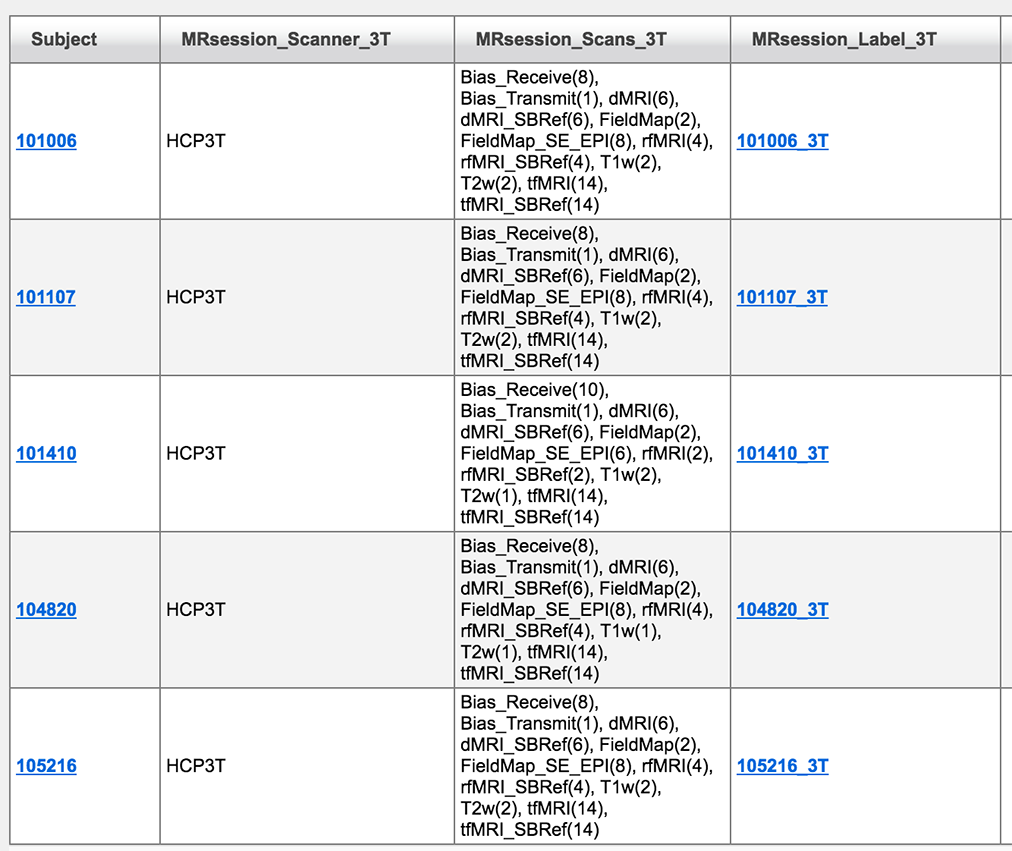
\includegraphics[width=\linewidth]{subject_scan_details.png}
\captionof{figure}{Subject Scan Details}
\label{fig:subject_scan_details}
\caption*{Extracted from \cite{DBConnectomeSite}}
\end{center}

\section{Processing}
The data was processed in the order PreFreeSurfer, FreeSurfer, PostFreeSurfer and fMRIVolume.
Two runs were made on CentOS6 and CentOS7. Tables \ref{tab:prefreesurfer_processing_centos7} and \ref{tab:prefreesurfer_processing_centos6} shows the details about processing subjects on CentOS7 and CentOS6 respectively.

\subsection{PreFreeSurfer}
\begin{center}
\tabulinesep=1.2mm
\begin{tabu} to \textwidth { | X[l] | X[l] | X[l] | }
  \hline
  Subject & Run no. & Time \\
  \hline
  101006 & RUN-1  & 0h and 56min \\
  \hline
  101107 & RUN-1  & 1h and 16min \\
  \hline
  101410 & RUN-1  & 1h and 27min \\
  \hline
  104820 & RUN-1  & 1h and 16min \\
  \hline
  105216 & RUN-1  & 1h and 36min \\
  \hline
  101006 & RUN-2  & 1h and 28min \\
  \hline
  101107 & RUN-2  & 1h and 26min \\
  \hline
  101410 & RUN-2  & 1h and 18min \\
  \hline
  104820 & RUN-2  & 1h and 10min \\
  \hline
  105216 & RUN-2  & 1h and 29min \\
  \hline
\end{tabu}
\captionof{table}{PreFreeSurfer Processing Details on CentOS7}
  \label{tab:prefreesurfer_processing_centos7}
\end{center}

\begin{center}
\tabulinesep=1.2mm
\begin{tabu} to \textwidth { | X[l] | X[l] | X[l] | }
  \hline
  Subject & Run no. & Time \\
  \hline
  101006 & RUN-1  & 1h and 17min \\
  \hline
  101107 & RUN-1  & 1h and 19min \\
  \hline
  101410 & RUN-1  & 1h and 09min \\
  \hline
  104820 & RUN-1  & 1h and 00min \\
  \hline
  105216 & RUN-1  & 1h and 17min \\
  \hline
  101006 & RUN-2  & 1h and 18min \\
  \hline
  101107 & RUN-2  & 1h and 16min \\
  \hline
  101410 & RUN-2  & 1h and 12min \\
  \hline
  104820 & RUN-2  & 0h and 58 min \\
  \hline
  105216 & RUN-2  & 1h and 31min \\
  \hline
\end{tabu}
\captionof{table}{PreFreeSurfer Processing Details on CentOS6}
  \label{tab:prefreesurfer_processing_centos6}
\end{center}

\begin{itemize}
  \item PreFreeSurfer
  \item FreeSurfer
  \item PostFreeSurfer
  \item fMRIVolume
\end{itemize}

\section{Evaluation}
\paragraph{File comparision across conditions using metrics}
\begin{itemize}
  \item NRMSE
  \item Dice
  \item Checksum
  \item Hardware
\end{itemize}
